% Options for packages loaded elsewhere
% Options for packages loaded elsewhere
\PassOptionsToPackage{unicode}{hyperref}
\PassOptionsToPackage{hyphens}{url}
%
\documentclass[
  ignorenonframetext,
  handout]{beamer}
\newif\ifbibliography
\usepackage{pgfpages}
\setbeamertemplate{caption}[numbered]
\setbeamertemplate{caption label separator}{: }
\setbeamercolor{caption name}{fg=normal text.fg}
\beamertemplatenavigationsymbolsempty
% remove section numbering
\setbeamertemplate{part page}{
  \centering
  \begin{beamercolorbox}[sep=16pt,center]{part title}
    \usebeamerfont{part title}\insertpart\par
  \end{beamercolorbox}
}
\setbeamertemplate{section page}{
  \centering
  \begin{beamercolorbox}[sep=12pt,center]{section title}
    \usebeamerfont{section title}\insertsection\par
  \end{beamercolorbox}
}
\setbeamertemplate{subsection page}{
  \centering
  \begin{beamercolorbox}[sep=8pt,center]{subsection title}
    \usebeamerfont{subsection title}\insertsubsection\par
  \end{beamercolorbox}
}
% Prevent slide breaks in the middle of a paragraph
\widowpenalties 1 10000
\raggedbottom
\AtBeginPart{
  \frame{\partpage}
}
\AtBeginSection{
  \ifbibliography
  \else
    \frame{\sectionpage}
  \fi
}
\AtBeginSubsection{
  \frame{\subsectionpage}
}
\usepackage{iftex}
\ifPDFTeX
  \usepackage[T1]{fontenc}
  \usepackage[utf8]{inputenc}
  \usepackage{textcomp} % provide euro and other symbols
\else % if luatex or xetex
  \usepackage{unicode-math} % this also loads fontspec
  \defaultfontfeatures{Scale=MatchLowercase}
  \defaultfontfeatures[\rmfamily]{Ligatures=TeX,Scale=1}
\fi
\usepackage{lmodern}

\usetheme[]{default}
\ifPDFTeX\else
  % xetex/luatex font selection
\fi
% Use upquote if available, for straight quotes in verbatim environments
\IfFileExists{upquote.sty}{\usepackage{upquote}}{}
\IfFileExists{microtype.sty}{% use microtype if available
  \usepackage[]{microtype}
  \UseMicrotypeSet[protrusion]{basicmath} % disable protrusion for tt fonts
}{}
\makeatletter
\@ifundefined{KOMAClassName}{% if non-KOMA class
  \IfFileExists{parskip.sty}{%
    \usepackage{parskip}
  }{% else
    \setlength{\parindent}{0pt}
    \setlength{\parskip}{6pt plus 2pt minus 1pt}}
}{% if KOMA class
  \KOMAoptions{parskip=half}}
\makeatother


\usepackage{longtable,booktabs,array}
\usepackage{calc} % for calculating minipage widths
\usepackage{caption}
% Make caption package work with longtable
\makeatletter
\def\fnum@table{\tablename~\thetable}
\makeatother
\usepackage{graphicx}
\makeatletter
\newsavebox\pandoc@box
\newcommand*\pandocbounded[1]{% scales image to fit in text height/width
  \sbox\pandoc@box{#1}%
  \Gscale@div\@tempa{\textheight}{\dimexpr\ht\pandoc@box+\dp\pandoc@box\relax}%
  \Gscale@div\@tempb{\linewidth}{\wd\pandoc@box}%
  \ifdim\@tempb\p@<\@tempa\p@\let\@tempa\@tempb\fi% select the smaller of both
  \ifdim\@tempa\p@<\p@\scalebox{\@tempa}{\usebox\pandoc@box}%
  \else\usebox{\pandoc@box}%
  \fi%
}
% Set default figure placement to htbp
\def\fps@figure{htbp}
\makeatother





\setlength{\emergencystretch}{3em} % prevent overfull lines

\providecommand{\tightlist}{%
  \setlength{\itemsep}{0pt}\setlength{\parskip}{0pt}}



 


\makeatletter
\@ifpackageloaded{tcolorbox}{}{\usepackage[skins,breakable]{tcolorbox}}
\@ifpackageloaded{fontawesome5}{}{\usepackage{fontawesome5}}
\definecolor{quarto-callout-color}{HTML}{909090}
\definecolor{quarto-callout-note-color}{HTML}{0758E5}
\definecolor{quarto-callout-important-color}{HTML}{CC1914}
\definecolor{quarto-callout-warning-color}{HTML}{EB9113}
\definecolor{quarto-callout-tip-color}{HTML}{00A047}
\definecolor{quarto-callout-caution-color}{HTML}{FC5300}
\definecolor{quarto-callout-color-frame}{HTML}{acacac}
\definecolor{quarto-callout-note-color-frame}{HTML}{4582ec}
\definecolor{quarto-callout-important-color-frame}{HTML}{d9534f}
\definecolor{quarto-callout-warning-color-frame}{HTML}{f0ad4e}
\definecolor{quarto-callout-tip-color-frame}{HTML}{02b875}
\definecolor{quarto-callout-caution-color-frame}{HTML}{fd7e14}
\makeatother
\makeatletter
\@ifpackageloaded{caption}{}{\usepackage{caption}}
\AtBeginDocument{%
\ifdefined\contentsname
  \renewcommand*\contentsname{Table of contents}
\else
  \newcommand\contentsname{Table of contents}
\fi
\ifdefined\listfigurename
  \renewcommand*\listfigurename{List of Figures}
\else
  \newcommand\listfigurename{List of Figures}
\fi
\ifdefined\listtablename
  \renewcommand*\listtablename{List of Tables}
\else
  \newcommand\listtablename{List of Tables}
\fi
\ifdefined\figurename
  \renewcommand*\figurename{Figure}
\else
  \newcommand\figurename{Figure}
\fi
\ifdefined\tablename
  \renewcommand*\tablename{Table}
\else
  \newcommand\tablename{Table}
\fi
}
\@ifpackageloaded{float}{}{\usepackage{float}}
\floatstyle{ruled}
\@ifundefined{c@chapter}{\newfloat{codelisting}{h}{lop}}{\newfloat{codelisting}{h}{lop}[chapter]}
\floatname{codelisting}{Listing}
\newcommand*\listoflistings{\listof{codelisting}{List of Listings}}
\makeatother
\makeatletter
\makeatother
\makeatletter
\@ifpackageloaded{caption}{}{\usepackage{caption}}
\@ifpackageloaded{subcaption}{}{\usepackage{subcaption}}
\makeatother

\usepackage{bookmark}
\IfFileExists{xurl.sty}{\usepackage{xurl}}{} % add URL line breaks if available
\urlstyle{same}
\hypersetup{
  pdftitle={Microeconomia},
  pdfauthor={ISCAL - IPL},
  hidelinks,
  pdfcreator={LaTeX via pandoc}}


\title{Microeconomia}
\subtitle{Optimização do Produtor: Mercado Concorrencial}
\author{ISCAL - IPL}
\date{}

\begin{document}
\frame{\titlepage}


\begin{frame}{Optimização do Produtor: Mercado Concorrencial}
\phantomsection\label{optimizauxe7uxe3o-do-produtor-mercado-concorrencial}
\begin{tcolorbox}[enhanced jigsaw, colback=white, colframe=quarto-callout-note-color-frame, arc=.35mm, leftrule=.75mm, rightrule=.15mm, opacityback=0, breakable, toprule=.15mm, bottomrule=.15mm, left=2mm]

\textbf{Objectivo:} Derivar a condição óptima de produção em
concorrência perfeita (\(P = Cmg\)), identificar os limiares de
rendibilidade e encerramento, e construir a curva de oferta individual.

\end{tcolorbox}
\end{frame}

\begin{frame}{Estruturas de Mercado}
\phantomsection\label{estruturas-de-mercado}
\footnotesize
\renewcommand{\arraystretch}{2.2}
\begin{tabular}{|c|c|c|c|c|c|}
\hline
\multicolumn{2}{|c|}{\cellcolor{blue!10} \multirow{2}{*}{\parbox{2cm}{\centering Estruturas de Mercado}}} &
\multicolumn{4}{c|}{\cellcolor{blue!10} N.º de vendedores} \\ \cline{3-6}
\multicolumn{2}{|c|}{\cellcolor{blue!10}} &
\cellcolor{blue!25} Muitos &
\cellcolor{blue!25} Poucos &
\cellcolor{blue!25} Dois &
\cellcolor{blue!25} Um \\ \hline
\cellcolor{blue!10} &
\cellcolor{blue!25} Muitos &
\cellcolor{green!25}\parbox{2.2cm}{\centering\textbf{Conc. Perfeita}} &
Oligopólio & Duopólio &
\cellcolor{yellow!30} Monopólio \\ \cline{2-6}
\cellcolor{blue!10} &
\cellcolor{blue!25} Poucos &
Oligopsónio &
\multicolumn{3}{c|}{\multirow{3}{*}{\parbox{4cm}{\centering Negociação Estratégica}}} \\ \cline{2-3}
\cellcolor{blue!10} &
\cellcolor{blue!25} Dois &
Duopsónio &
\multicolumn{3}{c|}{} \\ \cline{2-3}
\cellcolor{blue!10}\multirow{-4}{*}{\parbox{1.5cm}{\centering N.º de compradores}} &
\cellcolor{blue!25} Um &
Monopsónio &
\multicolumn{3}{c|}{} \\ \hline
\end{tabular}

Nesta aula estudamos \textbf{Concorrência Perfeita} --- a estrutura de
mercado de referência.
\end{frame}

\begin{frame}{Hipóteses da Concorrência Perfeita}
\phantomsection\label{hipuxf3teses-da-concorruxeancia-perfeita}
\begin{itemize}
\tightlist
\item
  \textbf{Mercado atomizado:} cada empresa representa uma fracção ínfima
  do mercado --- individualmente, ninguém influencia o preço
\item
  \textbf{Produto homogéneo:} os compradores são indiferentes entre
  fornecedores
\item
  \textbf{\emph{Price takers}:} cada empresa toma o preço de mercado
  \(P\) como dado (exógeno)
\item
  \textbf{Livre entrada e saída} do mercado
\item
  \textbf{Informação perfeita}
\end{itemize}

\begin{tcolorbox}[enhanced jigsaw, colback=white, colframe=quarto-callout-important-color-frame, arc=.35mm, leftrule=.75mm, rightrule=.15mm, opacityback=0, breakable, toprule=.15mm, bottomrule=.15mm, left=2mm]

A hipótese-chave é que a empresa não tem poder de mercado: para ela,
\(P\) é uma constante.

\end{tcolorbox}
\end{frame}

\begin{frame}{Maximização do Lucro}
\phantomsection\label{maximizauxe7uxe3o-do-lucro}
\[\max_{Q_i} \Pi_i = RT - CT = P \cdot Q_i - CT(Q_i)\]

\textbf{Condição de Primeira Ordem (CPO):}

\[\frac{d\Pi_i}{dQ_i} = P - \frac{dCT}{dQ_i} = 0 \;\Rightarrow\; \boxed{P = Cmg}\]

\textbf{Condição de Segunda Ordem (CSO):}

\[\frac{d^2\Pi_i}{dQ_i^2} = -\frac{dCmg}{dQ_i} < 0 \;\Rightarrow\; Cmg \text{ crescente}\]

A empresa produz onde \(P = Cmg\) \textbf{na zona crescente} de \(Cmg\)
--- que coincide com a Zona Económica de Exploração.
\end{frame}

\begin{frame}{Intuição: P = Cmg como Cmg = Bmg}
\phantomsection\label{intuiuxe7uxe3o-p-cmg-como-cmg-bmg}
\[P = Cmg\]

\begin{itemize}
\tightlist
\item
  \(P\) é o benefício marginal de produzir uma unidade adicional
  (receita por unidade vendida)
\item
  \(Cmg\) é o custo marginal de produzir essa unidade
\end{itemize}

\begin{itemize}
\tightlist
\item
  Se \(P > Cmg\): produzir mais aumenta o lucro → expandir
\item
  Se \(P < Cmg\): produzir mais reduz o lucro → contrair
\item
  Se \(P = Cmg\): lucro é máximo ✓
\end{itemize}

\begin{tcolorbox}[enhanced jigsaw, colback=white, colframe=quarto-callout-tip-color-frame, arc=.35mm, leftrule=.75mm, rightrule=.15mm, opacityback=0, breakable, toprule=.15mm, bottomrule=.15mm, left=2mm]

É novamente o princípio fundamental da racionalidade: \textbf{benefício
marginal = custo marginal}.

\end{tcolorbox}
\end{frame}

\begin{frame}{Lucro Gráfico: caso P \textgreater{} CTM}
\phantomsection\label{lucro-gruxe1fico-caso-p-ctm}
\begin{center}
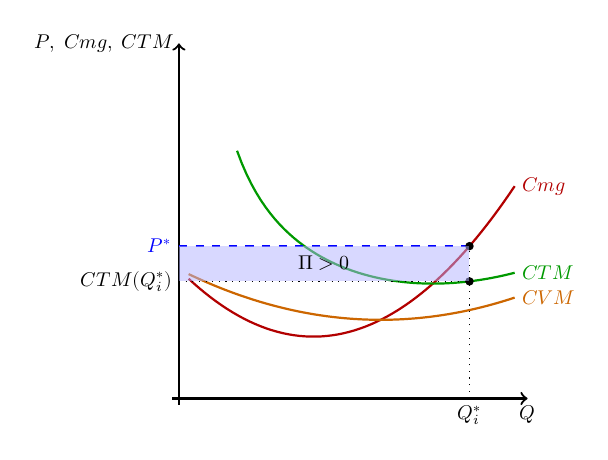
\begin{tikzpicture}[
  scale = 0.82,
  every node/.style = {scale = 0.72},
  declare function = {
    cv(\x) = \x - (1/4)*\x^2 + (1/25)*\x^3;
    ct(\x) = cv(\x) + 1;
    cmg(\x) = 1 - (1/2)*\x + (3/25)*\x^2;
    ctm(\x) = ct(\x)/\x;
    cvm(\x) = cv(\x)/\x;
  }
]
\def\pp{4.5}
\draw[->,thick] (-0.1,0) -- (5.4,0) node[below]{$Q$};
\draw[->,thick] (0,-0.1) -- (0,5.5) node[left]{$P,\;Cmg,\;CTM$};

\onslide<1->{
  \draw[red!70!black, thick, domain=0.15:5.2, variable=\x, samples=60]
    plot (\x,{2*cmg(\x)}) node[right]{$Cmg$};
  \draw[green!60!black, thick, domain=0.9:5.2, variable=\x, samples=60]
    plot (\x,{2*ctm(\x)}) node[right]{$CTM$};
  \draw[orange!80!black, thick, domain=0.15:5.2, variable=\x, samples=60]
    plot (\x,{2*cvm(\x)}) node[right]{$CVM$};
}
\onslide<2->{
  \draw[blue, thick, dashed] (0,{2*cmg(\pp)}) node[left]{$P^*$} -- (\pp,{2*cmg(\pp)});
  \draw[dotted] (\pp,0) node[below]{$Q_i^*$} -- (\pp,{2*cmg(\pp)})
    node[circle,fill,inner sep=1.5pt]{};
}
\onslide<3->{
  \draw[dotted] (0,{2*ctm(\pp)}) node[left]{$CTM(Q_i^*)$} -- (\pp,{2*ctm(\pp)})
    node[circle,fill,inner sep=1.5pt]{};
}
\onslide<4->{
  \fill[blue!30, opacity=0.5]
    (0,{2*ctm(\pp)}) rectangle (\pp,{2*cmg(\pp)});
  \node at ({\pp/2},{(2*cmg(\pp)+2*ctm(\pp))/2}) {$\Pi > 0$};
}
\end{tikzpicture}
\end{center}

\(\Pi^* = Q_i^* \cdot (P^* - CTM(Q_i^*)) > 0\) quando \(P^* > CTM\) ✓
\end{frame}

\begin{frame}{Lucro Gráfico: caso P \textless{} CTM mas P \textgreater{}
CVM}
\phantomsection\label{lucro-gruxe1fico-caso-p-ctm-mas-p-cvm}
\begin{center}
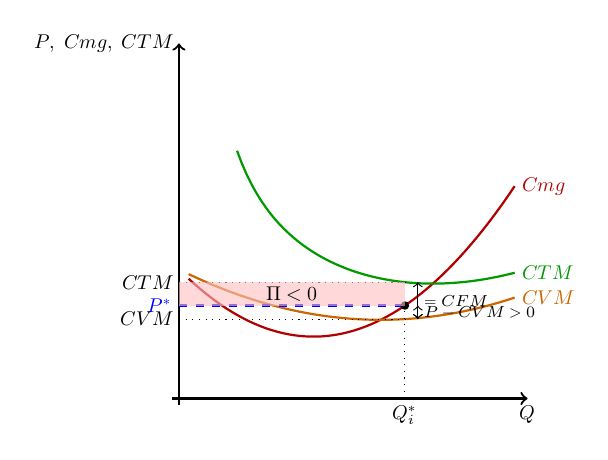
\begin{tikzpicture}[
  scale = 0.82,
  every node/.style = {scale = 0.72},
  declare function = {
    cv(\x) = \x - (1/4)*\x^2 + (1/25)*\x^3;
    ct(\x) = cv(\x) + 1;
    cmg(\x) = 1 - (1/2)*\x + (3/25)*\x^2;
    ctm(\x) = ct(\x)/\x;
    cvm(\x) = cv(\x)/\x;
  }
]
\def\pp{3.5}
\draw[->,thick] (-0.1,0) -- (5.4,0) node[below]{$Q$};
\draw[->,thick] (0,-0.1) -- (0,5.5) node[left]{$P,\;Cmg,\;CTM$};

\draw[red!70!black, thick, domain=0.15:5.2, variable=\x, samples=60]
  plot (\x,{2*cmg(\x)}) node[right]{$Cmg$};
\draw[green!60!black, thick, domain=0.9:5.2, variable=\x, samples=60]
  plot (\x,{2*ctm(\x)}) node[right]{$CTM$};
\draw[orange!80!black, thick, domain=0.15:5.2, variable=\x, samples=60]
  plot (\x,{2*cvm(\x)}) node[right]{$CVM$};

\onslide<2->{
  \draw[blue, thick, dashed] (0,{2*cmg(\pp)}) node[left]{$P^*$} -- (\pp,{2*cmg(\pp)});
  \draw[dotted] (\pp,0) node[below]{$Q_i^*$} -- (\pp,{2*cmg(\pp)})
    node[circle,fill,inner sep=1.5pt]{};
  \draw[dotted] (0,{2*ctm(\pp)}) node[left]{$CTM$} -- (\pp,{2*ctm(\pp)});
  \draw[dotted] (0,{2*cvm(\pp)}) node[left]{$CVM$} -- (\pp,{2*cvm(\pp)});
}
\onslide<3->{
  \fill[red!25, opacity=0.6]
    (0,{2*ctm(\pp)}) rectangle (\pp,{2*cmg(\pp)});
  \node at ({\pp/2},{(2*cmg(\pp)+2*ctm(\pp))/2}) {$\Pi < 0$};
}
\onslide<4->{
  % mostrar que P>CVM => prejudizo < CF => manter
  \draw[<->] (\pp+0.2,{2*cvm(\pp)}) -- (\pp+0.2,{2*ctm(\pp)})
    node[midway,right]{\footnotesize $= CFM$};
  \draw[<->] (\pp+0.2,{2*cmg(\pp)}) -- (\pp+0.2,{2*cvm(\pp)})
    node[midway,right]{\footnotesize $P - CVM > 0$};
}
\end{tikzpicture}
\end{center}

\(P > CVM\): a receita cobre os custos variáveis e parte dos fixos →
prejuízo \(< CF\) → \textbf{manter-se em funcionamento}
\end{frame}

\begin{frame}{Lucro e Prejuízo: Sistematização}
\phantomsection\label{lucro-e-prejuuxedzo-sistematizauxe7uxe3o}
\[\Pi = Q_i \cdot (P - CTM) = Q_i \cdot (P - CVM - CFM)\]

\begin{itemize}
\tightlist
\item
  \(P > CTM\): \textbf{lucro positivo} --- produzir ao nível \(P = Cmg\)
\item
  \(CVM < P < CTM\): \textbf{prejuízo} \(< CF\) --- vale a pena
  continuar a produzir (cobrem-se os custos variáveis e parte dos fixos)
\item
  \(P = CVM_{min}\): \textbf{limiar de encerramento} \(P_0\) ---
  indiferente entre produzir \(Q_0\) e encerrar
\item
  \(P < CVM_{min}\): \textbf{encerrar} --- prejuízo \(> CF\); encerrando
  perde-se apenas \(CF\)
\end{itemize}
\end{frame}

\begin{frame}{Os Dois Limiares}
\phantomsection\label{os-dois-limiares}
\begin{center}
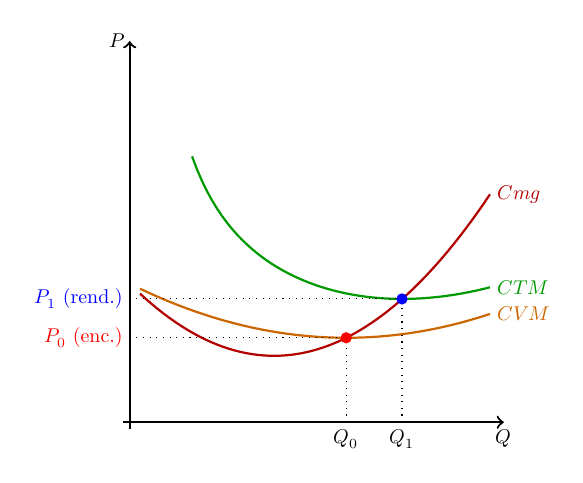
\begin{tikzpicture}[
  scale = 0.88,
  every node/.style = {scale = 0.72},
  declare function = {
    cv(\x) = \x - (1/4)*\x^2 + (1/25)*\x^3;
    ct(\x) = cv(\x) + 1;
    cmg(\x) = 1 - (1/2)*\x + (3/25)*\x^2;
    ctm(\x) = ct(\x)/\x;
    cvm(\x) = cv(\x)/\x;
  }
]
% mínimo CVM: Q=25/8=3.125
% mínimo CTM: Q=3.93 (aprox)
\def\penc{25/8}
\def\prend{3.93}

\draw[->,thick] (-0.1,0) -- (5.4,0) node[below]{$Q$};
\draw[->,thick] (0,-0.1) -- (0,5.5) node[left]{$P$};

\draw[red!70!black, thick, domain=0.15:5.2, variable=\x, samples=60]
  plot (\x,{2*cmg(\x)}) node[right]{$Cmg$};
\draw[green!60!black, thick, domain=0.9:5.2, variable=\x, samples=60]
  plot (\x,{2*ctm(\x)}) node[right]{$CTM$};
\draw[orange!80!black, thick, domain=0.15:5.2, variable=\x, samples=60]
  plot (\x,{2*cvm(\x)}) node[right]{$CVM$};

% limiar de encerramento
\draw[dotted] (0,{2*cvm(\penc)}) node[left]{\color{red}$P_0$ (enc.)} -- (\penc,{2*cvm(\penc)});
\draw[dotted] (\penc,0) node[below]{$Q_0$} -- (\penc,{2*cvm(\penc)})
  node[circle,fill=red,inner sep=2pt]{};

% limiar de rendibilidade
\draw[dotted] (0,{2*ctm(\prend)}) node[left]{\color{blue}$P_1$ (rend.)} -- (\prend,{2*ctm(\prend)});
\draw[dotted] (\prend,0) node[below]{$Q_1$} -- (\prend,{2*ctm(\prend)})
  node[circle,fill=blue,inner sep=2pt]{};

\end{tikzpicture}
\end{center}

\begin{itemize}
\tightlist
\item
  \(P_0 = CVM_{min}\): \textbf{limiar de encerramento} --- abaixo deste
  preço, a empresa fecha
\item
  \(P_1 = CTM_{min}\): \textbf{limiar de rendibilidade} --- acima deste
  preço, a empresa tem lucro \(> 0\)
\end{itemize}
\end{frame}

\begin{frame}{Curva de Oferta Individual}
\phantomsection\label{curva-de-oferta-individual}
A curva de oferta é o conjunto de pares \((Q, P)\) que constituem a
escolha óptima para cada preço:

\[S_i: \quad P = Cmg(Q_i) \quad \text{para } P \geq P_0 = CVM_{min}\]

\begin{center}
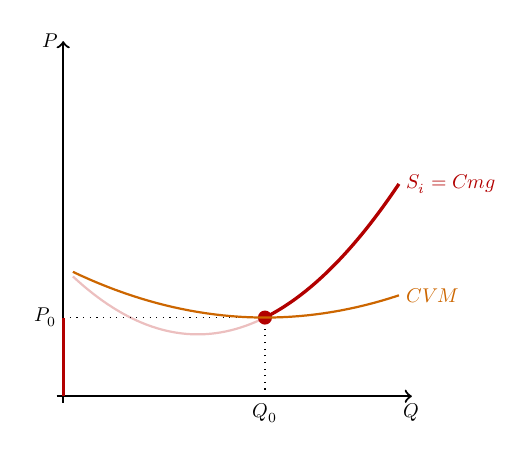
\begin{tikzpicture}[
  scale = 0.82,
  every node/.style = {scale = 0.72},
  declare function = {
    cmg(\x) = 1 - (1/2)*\x + (3/25)*\x^2;
    cvm(\x) = (1 - (1/4)*\x + (1/25)*\x^2);
  }
]
\def\penc{25/8}

\draw[->,thick] (-0.1,0) -- (5.4,0) node[below]{$Q$};
\draw[->,thick] (0,-0.1) -- (0,5.5) node[left]{$P$};

% parte inactiva (abaixo do limiar)
\draw[red!70!black, opacity=0.25, thick, domain=0.15:\penc, variable=\x, samples=40]
  plot (\x,{2*cmg(\x)});

% curva de oferta (acima do limiar)
\draw[red!70!black, very thick, domain=\penc:5.2, variable=\x, samples=40]
  plot (\x,{2*cmg(\x)}) node[right]{$S_i = Cmg$};

% eixo vertical abaixo do limiar (Q=0 para P<P0)
\draw[red!70!black, very thick] (0,0) -- (0,{2*cvm(\penc)});

% limiar
\draw[dotted] (0,{2*cvm(\penc)}) node[left]{$P_0$} -- (\penc,{2*cvm(\penc)});
\draw[dotted] (\penc,0) node[below]{$Q_0$} -- (\penc,{2*cvm(\penc)})
  node[circle,fill=red!70!black,inner sep=2.5pt]{};

\draw[orange!80!black, thick, domain=0.15:5.2, variable=\x, samples=40]
  plot (\x,{2*cvm(\x)}) node[right]{$CVM$};
\end{tikzpicture}
\end{center}
\end{frame}

\begin{frame}{Lei da Oferta}
\phantomsection\label{lei-da-oferta}
A curva de oferta tem \textbf{inclinação positiva}: se \(P\) sobe,
\(Q_i^*\) sobe --- e vice-versa.

\textbf{Porquê?} Na Zona Económica de Exploração, \(Cmg\) é
\textbf{crescente}. Para um preço mais alto, a igualdade \(P = Cmg\)
dá-se num nível de \(Q\) mais elevado.

\textbf{Fundamento último:} Lei dos Rendimentos Marginais Decrescentes
\(\Rightarrow\) \(Cmg\) crescente \(\Rightarrow\) curva de oferta
positivamente inclinada.

\begin{tcolorbox}[enhanced jigsaw, colback=white, colframe=quarto-callout-note-color-frame, arc=.35mm, leftrule=.75mm, rightrule=.15mm, opacityback=0, breakable, toprule=.15mm, bottomrule=.15mm, left=2mm]

A variação do \textbf{preço de venda} move ao longo da curva de oferta.
A variação de \textbf{factores exógenos} (preço dos inputs, tecnologia)
desloca a curva inteira.

\end{tcolorbox}
\end{frame}

\begin{frame}{Determinantes da Oferta}
\phantomsection\label{determinantes-da-oferta}
O preço de venda \(P\) é o único factor que move ao longo da curva. Os
restantes factores \textbf{deslocam} a curva:

\begin{itemize}
\tightlist
\item
  \textbf{Preços dos factores} \(w, r\) ↑ → custos sobem → oferta
  contrai (curva desloca para cima/esquerda)
\item
  \textbf{Tecnologia} \(A\) melhora → custos descem → oferta expande
  (curva desloca para baixo/direita)
\item
  \textbf{Preço de materiais} \(p_m\) ↑ → custos sobem → oferta contrai
\item
  \textbf{Número de empresas} ↑ → oferta de mercado expande
\end{itemize}
\end{frame}

\begin{frame}{Exemplo Resolvido}
\phantomsection\label{exemplo-resolvido}
\textbf{Dados:} \(CT = Q^3 - 60Q^2 + 1200Q + 1000\)

\begin{enumerate}
[a)]
\tightlist
\item
  Determine \(Cmg\), \(CVM\), \(CTM\).
\item
  Calcule os limiares de encerramento e rendibilidade.
\item
  Identifique a curva de oferta.
\item
  Se \(P = 330.75\), a empresa produz ou encerra? Tem lucro ou prejuízo?
\end{enumerate}
\end{frame}

\begin{frame}{Exemplo --- Resolução (a) e (b)}
\phantomsection\label{exemplo-resoluuxe7uxe3o-a-e-b}
\[Cmg = 3Q^2 - 120Q + 1200\]
\[CVM = Q^2 - 60Q + 1200 \qquad CTM = Q^2 - 60Q + 1200 + \tfrac{1000}{Q}\]

\textbf{Limiar de encerramento} --- mínimo de \(CVM\) (\(Cmg = CVM\)):

\[3Q^2 - 120Q + 1200 = Q^2 - 60Q + 1200 \;\Rightarrow\; 2Q^2 - 60Q = 0 \;\Rightarrow\; Q_0 = 30\]

\[P_0 = CVM(30) = 900 - 1800 + 1200 = \mathbf{300}\]

\textbf{Limiar de rendibilidade} --- mínimo de \(CTM\): por tentativas,

\(Q = 30.5\!:\)
\(CTM = (30.5)^2 - 60(30.5) + 1200 + \tfrac{1000}{30.5} = 930.25 - 1830 + 1200 + 32.79 \approx 333\)

\[P_1 \approx \mathbf{333}\]
\end{frame}

\begin{frame}{Exemplo --- Resolução (c) e (d)}
\phantomsection\label{exemplo-resoluuxe7uxe3o-c-e-d}
\textbf{Curva de oferta:}

\[S_i\!: \quad P = 3Q^2 - 120Q + 1200 \quad \text{para } P \geq 300\]

\textbf{Para \(P = 330.75\):} igualar \(P = Cmg\):

\[3Q^2 - 120Q + 1200 = 330.75 \;\Rightarrow\; 3Q^2 - 120Q + 869.25 = 0\]

\[Q = \frac{120 \pm \sqrt{14400 - 4 \times 3 \times 869.25}}{6} = \frac{120 \pm \sqrt{14400 - 10431}}{6} = \frac{120 \pm \sqrt{3969}}{6} = \frac{120 \pm 63}{6}\]

\(Q_a = 9.5\) (zona decrescente de \(Cmg\) --- inválido);
\(\quad Q^* = \dfrac{120+63}{6} = 30.5\)

\(CVM(30.5) = 930.25 - 1830 + 1200 = 300.25 < 330.75\) → produz

\(CTM(30.5) \approx 333 > 330.75\) → \textbf{prejuízo} (mas menor que
\(CF\)) ✓
\end{frame}

\begin{frame}{Exercícios --- Escolha Múltipla (1)}
\phantomsection\label{exercuxedcios-escolha-muxfaltipla-1}
\textbf{1.} Uma empresa em concorrência perfeita tem \(Cmg = 2Q + 4\) e
\(CVM_{min} = 4\) (para \(Q = 0\)). Se o preço de mercado for
\(P = 14\), qual a produção óptima?

\begin{enumerate}
[a)]
\tightlist
\item
  \(Q^* = 4\)
\item
  \(Q^* = 5\) ✓
\item
  \(Q^* = 7\)
\item
  A empresa encerra.
\end{enumerate}

\textbf{Solução:}
\(P = Cmg \Rightarrow 14 = 2Q + 4 \Rightarrow Q^* = 5\).

Verificação de encerramento: \(P = 14 > CVM_{min} = 4\) → não encerra ✓
\end{frame}

\begin{frame}{Exercícios --- Escolha Múltipla (2)}
\phantomsection\label{exercuxedcios-escolha-muxfaltipla-2}
\textbf{2.} Para uma empresa em concorrência perfeita com
\(CT = 2Q^2 + 6Q + 50\), qual o limiar de encerramento?

\begin{enumerate}
[a)]
\tightlist
\item
  \(P_0 = 6\) ✓
\item
  \(P_0 = 10\)
\item
  \(P_0 = 50\)
\item
  \(P_0 = 56\)
\end{enumerate}

\textbf{Solução:} \(CV = 2Q^2 + 6Q\); \(CVM = 2Q + 6\).

\(CVM\) é crescente para todo \(Q > 0\) (é uma recta), logo o mínimo é
em \(Q \to 0\): \(CVM_{min} = 6\).

Verificação: \(Cmg = 4Q + 6\).
\(Cmg = CVM \Rightarrow 4Q + 6 = 2Q + 6 \Rightarrow Q = 0\).
\(CVM(0) = 6\) ✓

\(P_0 = 6\).
\end{frame}

\begin{frame}{Exercício de Desenvolvimento}
\phantomsection\label{exercuxedcio-de-desenvolvimento}
\textbf{Enunciado:} Uma empresa em concorrência perfeita tem
\(CT = Q^3 - 9Q^2 + 30Q + 18\).

\begin{enumerate}
[a)]
\item
  Determine \(Cmg\), \(CVM\) e \(CTM\).
\item
  Calcule os limiares de encerramento e rendibilidade.
\item
  Se \(P = 12\), qual a produção óptima? Tem lucro ou prejuízo? Deve
  manter-se em funcionamento?
\item
  Escreva a expressão da curva de oferta desta empresa.
\end{enumerate}
\end{frame}

\begin{frame}{Solução --- Desenvolvimento (a) e (b)}
\phantomsection\label{soluuxe7uxe3o-desenvolvimento-a-e-b}
\[Cmg = 3Q^2 - 18Q + 30, \quad CVM = Q^2 - 9Q + 30, \quad CTM = Q^2 - 9Q + 30 + \tfrac{18}{Q}\]

\textbf{Limiar de encerramento} (\(Cmg = CVM\)):

\[3Q^2 - 18Q + 30 = Q^2 - 9Q + 30 \;\Rightarrow\; 2Q^2 - 9Q = 0 \;\Rightarrow\; Q_0 = 4.5\]

\[P_0 = CVM(4.5) = 20.25 - 40.5 + 30 = \mathbf{9.75}\]

\textbf{Limiar de rendibilidade} (\(Cmg = CTM\)):

\[3Q^2 - 18Q + 30 = Q^2 - 9Q + 30 + \tfrac{18}{Q} \;\Rightarrow\; 2Q^3 - 9Q^2 - 18 = 0\]

Por tentativas: \(Q = 4.87 \Rightarrow CTM(4.87) \approx 13.59\).

\[P_1 \approx \mathbf{13.59}\]
\end{frame}

\begin{frame}{Solução --- Desenvolvimento (c) e (d)}
\phantomsection\label{soluuxe7uxe3o-desenvolvimento-c-e-d}
\textbf{Para \(P = 12\):}
\(P = Cmg \Rightarrow 3Q^2 - 18Q + 30 = 12 \Rightarrow 3Q^2 - 18Q + 18 = 0 \Rightarrow Q^2 - 6Q + 6 = 0\)

\[Q = \frac{6 \pm \sqrt{36 - 24}}{2} = \frac{6 \pm \sqrt{12}}{2} = 3 \pm \sqrt{3}\]

\(Q_a = 3 - \sqrt{3} \approx 1.27\) (zona decrescente de \(Cmg\) ---
inválido)

\(Q^* = 3 + \sqrt{3} \approx 4.73\)

\(CVM(4.73) = 22.37 - 42.57 + 30 = 9.80\)

\(CTM(4.73) = 9.80 + 18/4.73 = 9.80 + 3.81 = 13.61\)

\(P = 12 > P_0 = 9.75\) → \textbf{mantém-se em funcionamento} ✓

\(P = 12 < P_1 \approx 13.59\) → \textbf{tem prejuízo} (mas inferior a
\(CF = 18\)) ✓

\textbf{Curva de oferta:} \(S_i\!: P = 3Q^2 - 18Q + 30\) para
\(P \geq 9.75\)
\end{frame}




\end{document}
